\documentclass{article}
\usepackage[T1]{fontenc}
% Official CoRL typography; preprint exposes authors without claiming acceptance.
\usepackage[preprint]{corl_2026}
\usepackage{graphicx}
\usepackage{booktabs}
\title{AHOPPA: Agentic Humanoid Operation through Perception, Planning, and Action}
\author{Kingston Kuan$^{1}$ \qquad Samuel J Chew$^{2}$ \qquad Brandon Ong$^{1}$ \\ $^{1}$Hebbian Robotics \qquad $^{2}$Carnegie Mellon University}
\begin{document}
\maketitle
\hypersetup{pdftitle={AHOPPA: Agentic Humanoid Operation through Perception, Planning, and Action},pdfauthor={Kingston Kuan, Samuel J Chew, and Brandon Ong},pdfsubject={Online humanoid operation with frontier models}}
\begin{center}\small\url{https://hebbian-robotics.github.io/AHOPPA/}\end{center}

\begin{abstract}
Humanoid operation couples navigation, contact and completion judgments while
physics continues during inference. We report results obtained in the last few
weeks following frontier model releases. AHOPPA connects multimodal models to a
fixed SONIC controller on a simulated Unitree G1. Cameras, a map and revisable
plans guide head/wrist and locomotion commands to inspect four drawers, close
open ones and return home. Across 64 episodes with four models at two reasoning
efforts, GPT-6 Astra succeeded in 12/14 task attempts, taking 615 to 1492\,s.
Independent evaluation exposes falls, timeouts and incorrect completion claims.
\end{abstract}
\keywords{Humanoid control, multimodal agents, online evaluation}

\begin{figure}[h]
  \centering
  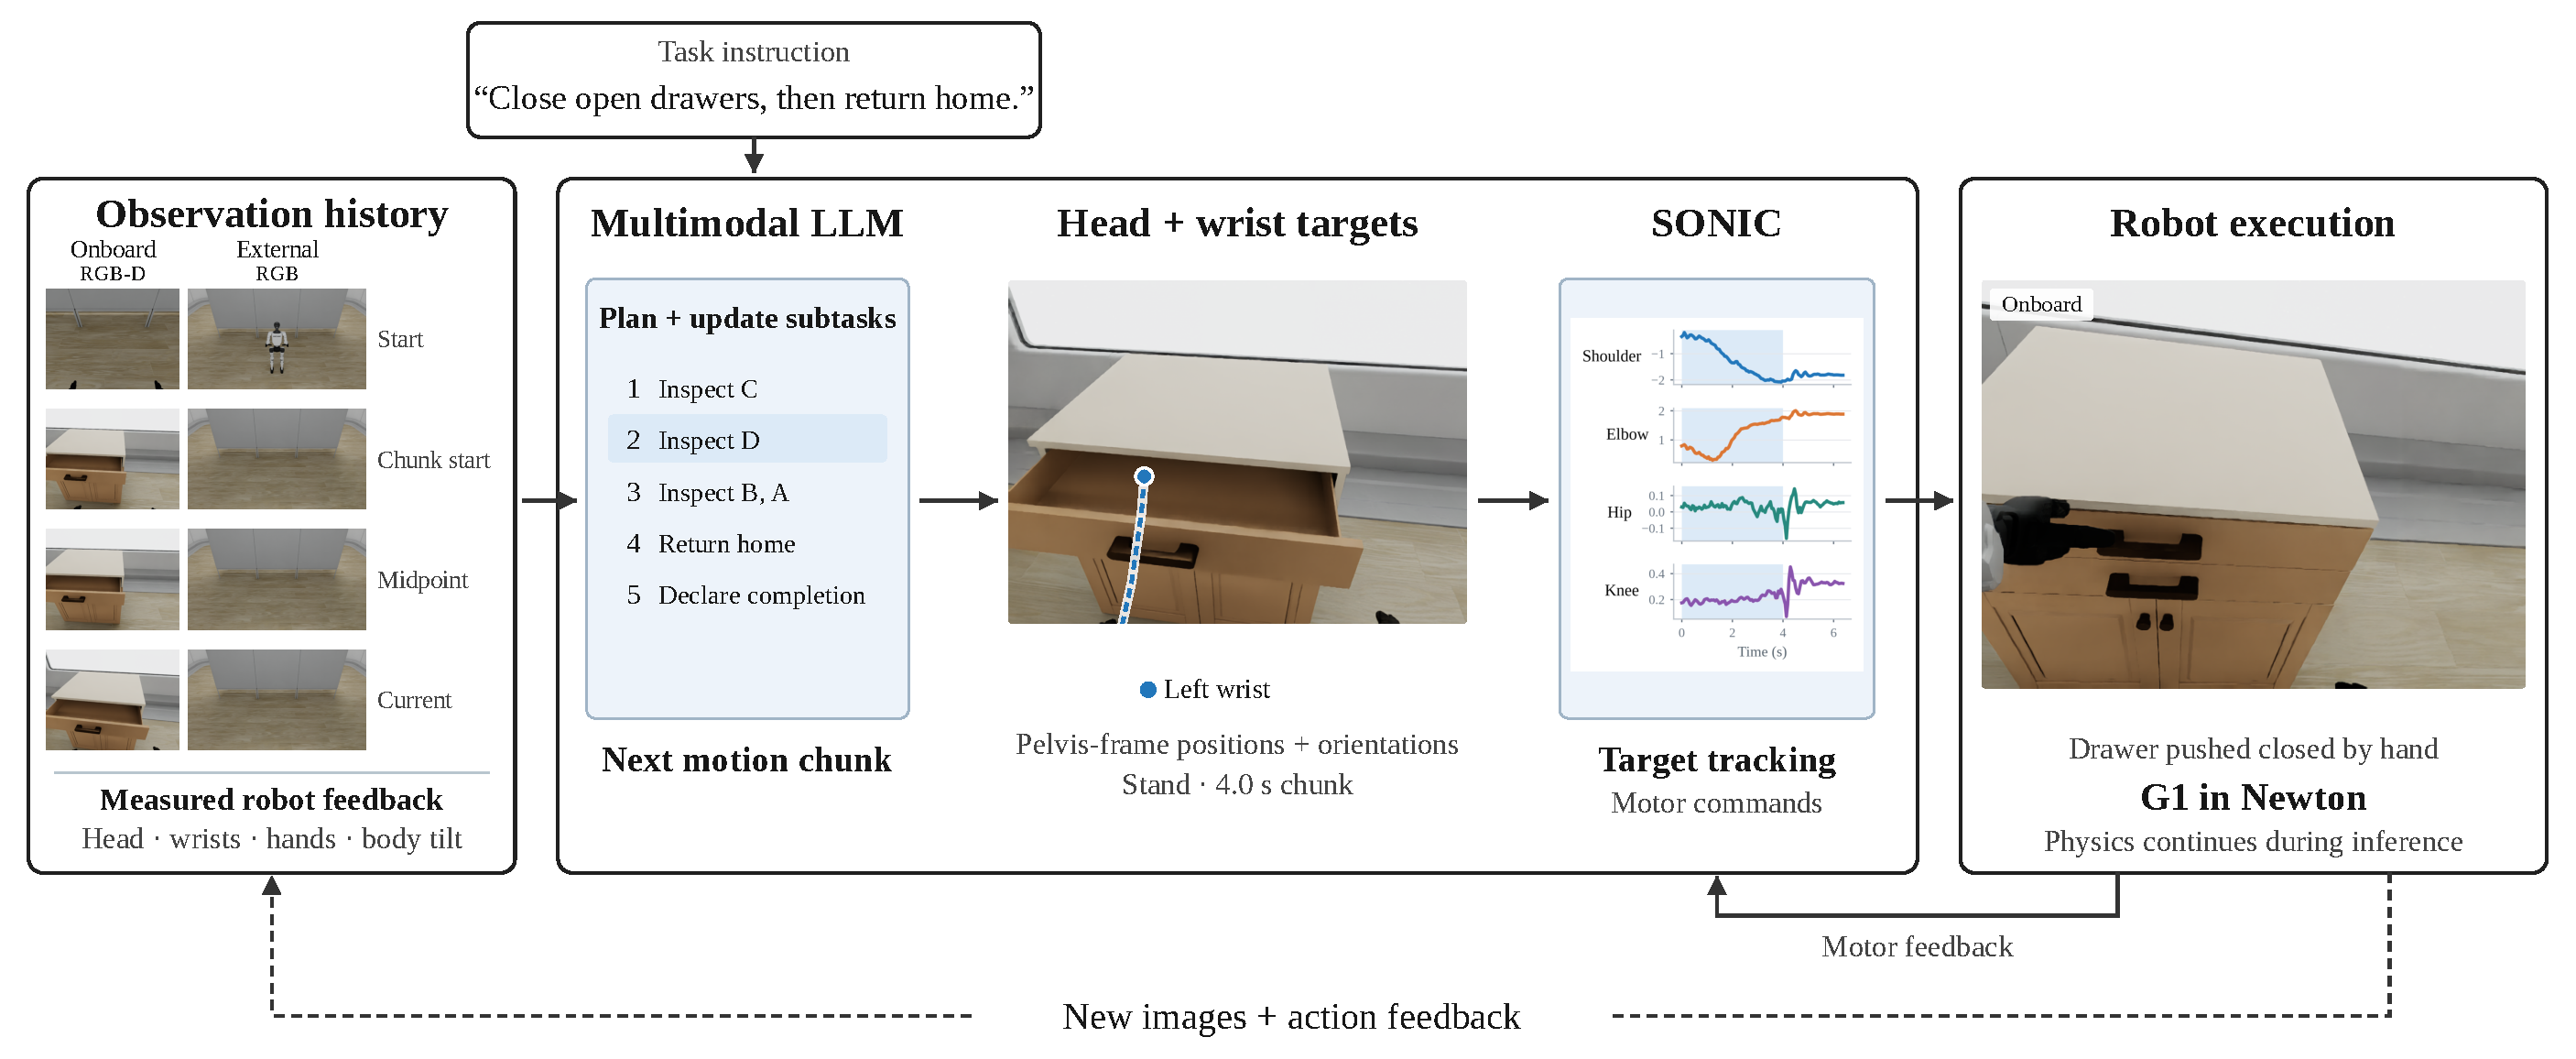
\includegraphics[width=\linewidth]{../docs/figures/system-overview.pdf}
  \par\smallskip
  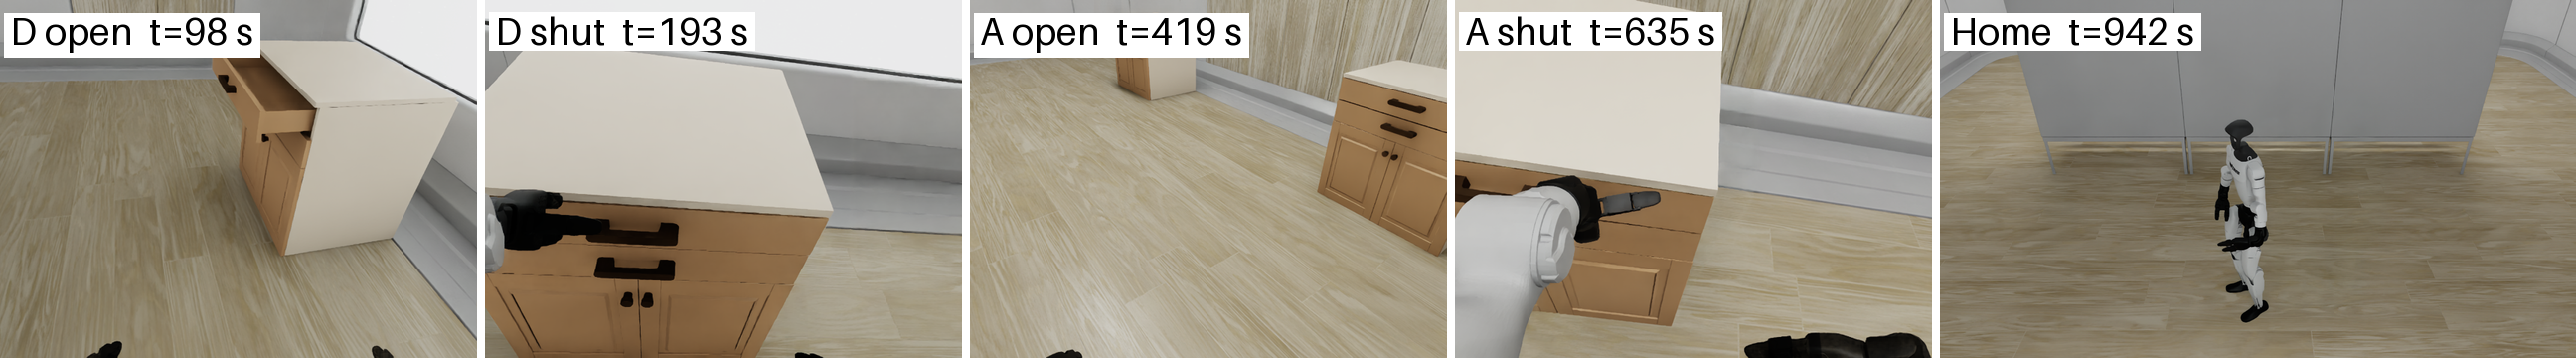
\includegraphics[width=\linewidth]{figures/astra-episode-sequence.png}
  \caption{Top: the agent loop with recorded inputs and commands. Bottom:
  selected original observations from the same successful Astra (low) episode,
  with A and D initially open. Labels give elapsed seconds; the completion
  declaration followed at 955\,s.}
  \label{fig:overview}
\end{figure}

\section{Online humanoid operation}
Room-scale humanoid operation couples navigation, inspection, contact and
stopping while physics continues during inference. We test frontier models
through numerical SONIC references~\citep{sonic2026}. Prior work spans skills,
code, feedback and spatial or learned action representations~\citep{saycan2022,homebody2026,promptplanperform2024,codeaspolicies2022,choi2026hugo,innermonologue2022,pivot2024,voxposer2023,sayplan2023,rekep2025,rt22023}.
We measure task completion, reasoning-effort tradeoffs and failures without a
task skill library.

\section{Interface, task and evaluation}
\textbf{Interface.} The model receives onboard RGB-D, external RGB, robot
kinematics, depth queries, a map, a revisable plan and feedback. It sends
head/wrist keyframes, walking/posture commands and binary hand presets to SONIC
(Fig.~\ref{fig:overview}). Drawer joint positions, contacts and scores are
withheld; no task skills are supplied.

\textbf{Task.} Four Sektion cabinets~\citep{isaaclab2026cabinet} stand in
NVIDIA's Simple Room~\citep{nvidia2026warehouseassets,nvidia2026assetlicense}:
A and B behind 2.1\,m lockers~\citep{nvidia2026simready}, C and D behind home.
No drawer front is visible initially. Newton~\citep{newton2025} in
Isaac Lab~\citep{isaaclab2025} supplies contact physics with passive drawers
and flat-ground support. Eight conditions vary which drawers start 0.20\,m open under the same
instruction.

\textbf{Scoring.} Closed means within 2\,cm of shut and still for 1\,s.
Success requires all drawers closed, a supported standing hold within 25\,cm
of home and the model's completion declaration. Force sensors distinguish hand
pushes from other contact. We record physical completion, inspection,
disturbance, falls, timeouts and API errors separately.

\textbf{Protocol.} After pilots, we froze the setup, prompts, evaluator, source
and 1800\,s budget. GPT-6.1 Sol, GPT-6 Astra, Claude Opus 5.5 and Gemini 4 Argon
each attempted every condition once at low and high effort, following a seeded
condition schedule.

\section{Results}


\begin{table}[t]
  \centering
  \small
  \setlength{\tabcolsep}{3pt}
  \begin{tabular}{lccccccccc}
\toprule
Model & Success & Physical & Closed & Seen & False & Control & Est. \$ & Episode (s) & Decision (s) \\
\midrule
Astra (low) & 6/7 & 6 & 9 & 5 & 0 & 1/1 & 9.30 / 10.57 & 817 / 926 & 9.2 / 9.4 \\
Astra (high) & 6/7 & 6 & 8 & 6 & 0 & 0/1 & 7.65 / 8.78 & 998 / 1145 & 21.4 / 21.8 \\
Sol (low) & 4/7 & 4 & 4 & 5 & 1 & 0/1 & 1.72 / 1.96 & 829 / 940 & 10.4 / 10.4 \\
Sol (high) & 3/7 & 5 & 9 & 6 & 0 & 0/1 & 1.74 / 1.59 & 1235 / 1162 & 21.5 / 21.8 \\
Opus (low) & 2/7 & 3 & 5 & 4 & 2 & 1/1 & 4.78 / 6.23 & 762 / 1028 & 13.2 / 13.5 \\
Opus (high) & 3/7 & 3 & 6 & 3 & 1 & 1/1 & 7.22 / 8.36 & 1392 / 1563 & 36.1 / 34.5 \\
Gemini (low) & 0/7 & 0 & 0 & 1 & 0 & 0/1 & 1.29 / --$^{*}$ & 737 / --$^{*}$ & 32.3 / --$^{*}$ \\
Gemini (high) & 0/7 & 0 & 2 & 1 & 0 & 0/1 & 1.59 / --$^{*}$ & 1332 / --$^{*}$ & 136.7 / --$^{*}$ \\
\bottomrule
\end{tabular}

  \caption{Seven scheduled task attempts per row; all-closed controls are separate.
  Other counts use completed episodes. \emph{Physical}: closed, home, upright;
  \emph{Seen}: all fronts viewed; \emph{False}: declarations without physical
  completion. Pairs show all / successful attempts: mean cost and episode time,
  median per-attempt median decision latency. Costs use published
  rates~\citep{openai2026pricing,anthropic2026pricing,google2026pricing}.
  $^{*}$: no successful attempt observed. API-error starts stay in denominators.}
  \label{tab:results}
\end{table}
\textbf{Task completion.} Astra completed 12/14 task attempts in 615 to
1492\,s, combining inspection, hand contact and return home
(Fig.~\ref{fig:overview}). All 43 closures were by hand; no initially closed
drawer was disturbed.

\textbf{Reasoning effort and efficiency.} High effort lengthened decisions
without consistent success gains. Astra high cost less despite more output
tokens: cached reads covered 50\% of its input, versus 29\% at low.

\textbf{Failure modes and timing.} Fifteen of 51 completed task starts ended
in falls, one before any model command; eight timed out and four declarations
lacked physical completion. Only 17/58 completed episodes, including 7 task
successes, met the 100\,ms physics-lag limit; median peak lag was 192\,ms.
The results retain timing-limited episodes. Falls rarely followed lag spikes.

\textbf{Limits.} One simulated layout, drawer interaction and trial per
model/effort/condition limit generalization. Friction, damping and ground support
are modeling choices. Reliability, gains and transfer need repeated trials,
older-model baselines and hardware experiments.

\clearpage
\bibliography{../docs/references}
\end{document}
